\documentclass{article}
\usepackage[utf8]{inputenc}
\usepackage{longtable}
\usepackage{gensymb}
\usepackage{graphicx}
\usepackage{siunitx}
\usepackage{caption}
\usepackage[colorlinks,bookmarks=false,citecolor=blue,linkcolor=blue,urlcolor=blue]{hyperref}
\usepackage{relsize}
\usepackage{amsmath}
\usepackage{amssymb}
\usepackage{bm}

\begin{document}
\begin{titlepage}
\begin{center}

\includegraphics[scale=0.12]{document/niser.png}
\line(1,0){340}\\
[2mm]
\begin{large}
\textbf{\huge The Michelson Interferometer}\\ 
\end{large}
\line(1,0){200}\\
[5cm]
\large MAITREY SHARMA\\
\small (1911093)\\
[3.5cm]
Third Year Integrated M.Sc.\\
\textbf{School of Physical Sciences}\\
\textbf{National Institute of Science Education and Research, Bhubaneshwar}\\
\small August 19, 2021
\end{center} 
\end{titlepage}
\newpage
\section{Aim}
\begin{itemize}
    \item Alignment of Michelson’s Interferometer using He - Ne laser to observe concentric circular fringes.
    \item Measurement of the wavelength of He-Ne Laser and Na lamp using circular fringes.
    \item Study of fringes of equal inclination and equal thickness using Na lamp.
\end{itemize}
\section{Apparatus}
\begin{enumerate}
    \item Michelson's Interferometer
    \item He-Ne Laser
    \item Na lamp
    \item Screen.
\end{enumerate}

\section{Introduction}
\noindent \textbf{Interference} is a phenomenon in which two waves superpose to form a resultant wave of greater, lower, or the same amplitude. \textbf{Interferometers} are devices that extract information from interference. These are basic optical tools used to precisely measure wavelength, distance, index of refraction, and temporal coherence of optical beams. They are also widely used in science and industry for the measurement of microscopic displacements, refractive index changes and surface irregularities. In the case with most interferometers, light from a single source is split into two beams that travel in different optical paths, which are then combined again to produce interference.
\par
\noindent
The \textbf{Michelson interferometer} is an amplitude-splitting interferometer devised by Albert Michelson. It became well-known for its use by Michelson and Edward Morley in the famous Michelson–Morley experiments in 1887 in a configuration which would have detected the Earth's motion through the supposed luminiferous ether that most physicists at the time believed was the medium in which light waves propagated. The null result of that experiment essentially disproved the existence of such an ether, leading eventually to the special theory of relativity and the revolution in physics at the beginning of the twentieth century. The Laser Interferometer Gravitational-Wave Observatory (LIGO) is also an application of the Michelson interferometer which made the first direct observation of gravitational waves. It is still an important instrument in today's laboratories and it is being widely used as an instrument for measuring the wavelength of an unknown light source, to measure extremely small distance and for investigating optical media.

\section{Construction}
\noindent
The Michelson interferometer consists of two highly polished mirrors $M_1$ and $M_2$. Two glass plates beam splitter ($BS$) and compensatory glass plate ($CP$), are placed parallel to each 
other between the mirrors at an angle of $45\degree$. The rear side of glass plate $BS$ is semi-silvered such that the light from a source is equally reflected and transmitted by it. In this way division of amplitude takes place.
\begin{figure}[h!]
    \centering
    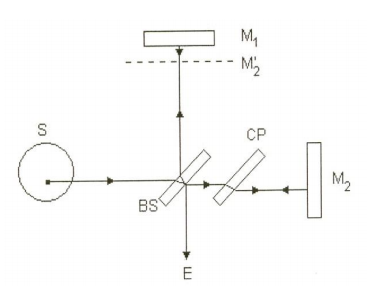
\includegraphics{Figures/Construction of michelson intef.png}
    \caption{Construction of Michelson's interferometer}
    \label{fig:construction}
\end{figure}
\par
\noindent
A monochromatic light of wavelength $\lambda$ falling on $BS$ is half reflected towards the mirror $M_1$ and the other half is transmitted towards mirror $M_2$. After splitting, the two rays are reflected back by the mirrors $M_1$ and $M_2$ and return to the plate $BS$. The ray reflected from $M_1$ is transmitted through $BS$ and the ray reflected from $M_2$ is reflected again by $BS$. The two rays coming from the two mirrors interfere and fringes are observed on a screen (for laser) or by naked eye (Na lamp) at E.
\section{Theory}
\noindent The wave reflected from $M_1$ and entering the eye crosses $BS$ twice. 
However the path of the other wave falling on the mirror $M_2$, in the absence of compensating 
plate $CP$, travels totally in air. Thus an extra \textbf{optical path} $2(\mu - 1)t$ is introduced where, $t$ is 
the thickness of the plate and $\mu$ is the refractive index of the $BS$ plate for the 
monochromatic light used. Thus, the two waves will interfere constructively or destructively as per the following conditions of path difference, $\Delta$:
\begin{center}
    $\Delta = 2 n \lambda /2 = n \lambda$ \hspace{1cm} (for maxima, $n$ is an integer)\\
    $\Delta = (2n + 1) \lambda /2$ \hspace{1cm} (for minima, $n$ is an integer)
\end{center}
\par
\noindent
Depending upon the nature of the air film, the fringes formed in the interferometer can be of various geometries. \textbf{Concentric circular fringes} or \textbf{fringes of equal thickness} are obtained when the air film is parallel as shown in figure~(\ref{fig:circular_fringes}). $M'_2$ is the virtual image of $M_2$ and it is parallel to $M_1$. $L_1$ and $L_2$ are the virtual images of $L$ formed by $M_1$ and $M'_2$ and are coherent. Let $d$ be the distance between $M_1$ and $M'_2$, therefore the distance between $L_1$ and $L_2$ is $2d$. Let $\theta$ be the angle between the incident beam originated at $P$ and the reflected beams from $M_1$ and $M'_2$. Then path difference between light beams from points $P'$ and $P''$ is $2d \cos{\theta}$. A maximum (bright fringe) will be formed when $2d \cos{\theta} = n \lambda$. Each circular ring corresponds to a particular value of $\theta$.
\begin{figure}[h!]
    \centering
    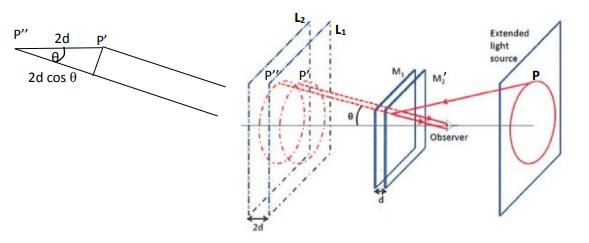
\includegraphics[scale = 0.7]{Figures/form of circl fringes.png}
    \caption{Formation of circular fringes}
    \label{fig:circular_fringes}
\end{figure}
\par
\noindent
When $M_1$ and virtual image $M'_2$ are inclined to each other, the film enclosed is wedge shaped. Then \textbf{curved fringes} can be observed as shown in figure~(\ref{fig:curved_fringes}). These are also known as \textbf{fringes of equal thickness}.
\begin{figure}[h!]
    \centering
    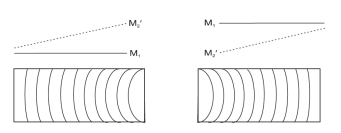
\includegraphics{Figures/form. of curved fring.png}
    \caption{Formation of curved fringes}
    \label{fig:curved_fringes}
\end{figure}
\par
\noindent
When $M_1$ and virtual image $M'_2$ intersect, straight line fringes are obtained around the point of intersection.
\begin{figure}[h!]
    \centering
    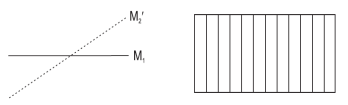
\includegraphics{Figures/form of strg lin fring.png}
    \caption{Formation of straight line fringes}
    \label{fig:straight_fringes}
\end{figure}
\par
\noindent
Circular fringes are used to determine the wavelength of the source of light. For a given separation of $d$ between the mirrors $M_1$ and $M_2$ and normal incidence ($\theta = 0$), the path 
difference is given as $2d = n \lambda$. If one mirror is moved by a distance $\Delta d$ and $N$ number of rings appear/disappear at the center, then the path difference after moving the mirror is given as
\begin{equation}
\label{eq00}
    2(d + \Delta d) = (n + N) \lambda
\end{equation}
\par
\noindent
Hence, 
\begin{equation}
    \boxed{\mathbf{\lambda = 2 (\Delta d)/ N}}
\end{equation}

\section{Experimental Setup}
\begin{figure}[h!]
    \centering
    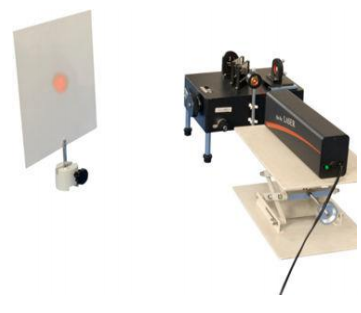
\includegraphics[scale = 0.8]{Figures/laser setup.png}
    \caption{Setup with Laser as the source}
    \label{fig:laser_setup}
\end{figure}
\begin{figure}[h!]
    \centering
    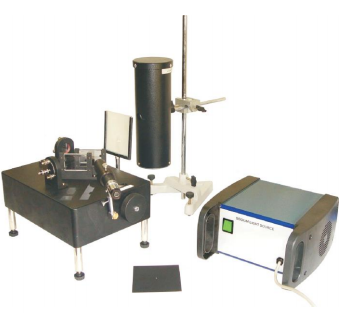
\includegraphics[scale = 1]{Figures/nalamp setup.png}
    \caption{Setup with Na lamp as source}
    \label{fig:lamp_setup}
\end{figure}
\begin{figure}[h!]
    \centering
    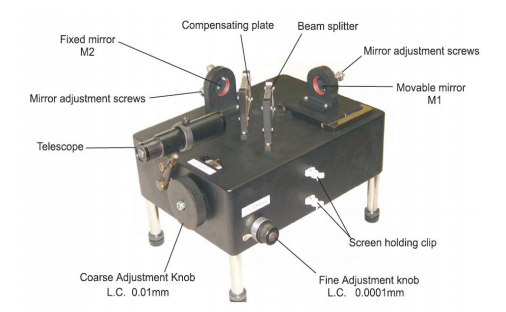
\includegraphics[scale = 0.90]{Figures/schematics.png}
    \caption{Schematics of Michelson interferometer}
    \label{fig:schematics}
\end{figure}
\section{Observations}
\begin{enumerate}
    \item Least count of coarse adjustment knob = \SI{0.01}{\milli\metre}
    \item Least count of fine adjustment knob = \SI{0.0001}{\milli\metre}
\end{enumerate}
\begin{table}[h!]
\centering
\caption{\textbf{Data for He-Ne Laser} \\ Initial position of gauge, $d_1 = \SI{0.0341}{\milli\metre}$}
\begin{tabular}{cccccc}
\hline
\hline
\textbf{\#} & \begin{tabular}[c]{@{}c@{}} \textbf{No. of rings} \\ N \end{tabular} & \begin{tabular}[c]{@{}c@{}} \textbf{Coarse} \\ \textbf{adjustment} \\ \textbf{reading},\\ m\end{tabular} & \begin{tabular}[c]{@{}c@{}} \textbf{Fine} \\ \textbf{adjustment} \\ \textbf{reading},\\ n\end{tabular} & \begin{tabular}[c]{@{}c@{}} \boldmath $d_2$ \\ (mm)\end{tabular} & \begin{tabular}[c]{@{}c@{}} \boldmath $\Delta d$ \\ (\boldmath $d_2 - d_1$) \\ (mm)\end{tabular} \\ \hline \hline
1      & 10                                                           & 3                                                                              & 73                                                                           & 0.0373                                            & 0.0032                                              \\ \hline
2      & 20                                                           & 4                                                                              & 8                                                                            & 0.0408                                            & 0.0067                                              \\ \hline
3      & 30                                                           & 4                                                                              & 42                                                                           & 0.0442                                            & 0.0101                                              \\ \hline
4      & 40                                                           & 4                                                                              & 68                                                                           & 0.0468                                            & 0.0127                                              \\ \hline
5      & 50                                                           & 5                                                                              & 6                                                                            & 0.0506                                            & 0.0165                                              \\ \hline
6      & 60                                                           & 5                                                                              & 38                                                                           & 0.0538                                            & 0.0197                                              \\ \hline
7      & 70                                                           & 5                                                                              & 63                                                                           & 0.0563                                            & 0.0222                                              \\ \hline
8      & 80                                                           & 5                                                                              & 96                                                                           & 0.0596                                            & 0.0255                                              \\ \hline
9      & 90                                                           & 6                                                                              & 29                                                                           & 0.0629                                            & 0.0288                                              \\ \hline
10     & 100                                                          & 6                                                                              & 56                                                                           & 0.0656                                            & 0.0315                                              \\ \hline
11     & 110                                                          & 6                                                                              & 86                                                                           & 0.0686                                            & 0.0345                                              \\ \hline
12     & 120                                                          & 7                                                                              & 19                                                                           & 0.0719                                            & 0.0378                                              \\ \hline
\end{tabular}
\label{Tab:He-Ne}
\end{table}
\begin{table}[h!]
\centering
\caption{\textbf{Data for Na Lamp} \\ Initial position of gauge, $d_1 = \SI{0.0165}{\milli\metre}$}
\begin{tabular}{cccccc}
\hline
\hline
\textbf{\#} & \begin{tabular}[c]{@{}c@{}} \textbf{No. of rings} \\ N \end{tabular} & \begin{tabular}[c]{@{}c@{}} \textbf{Coarse} \\ \textbf{adjustment} \\ \textbf{reading},\\ m\end{tabular} & \begin{tabular}[c]{@{}c@{}} \textbf{Fine} \\ \textbf{adjustment} \\ \textbf{reading},\\ n\end{tabular} & \begin{tabular}[c]{@{}c@{}} \boldmath $d_2$ \\ (mm)\end{tabular} & \begin{tabular}[c]{@{}c@{}} \boldmath $\Delta d$ \\ (\boldmath $d_2 - d_1$) \\ (mm)\end{tabular} \\ \hline \hline
1      & 10                                                           & 1                                                                              & 90                                                                           & 0.0190                                            & 0.0025                                              \\ \hline
2      & 20                                                           & 2                                                                              & 12                                                                            & 0.0212                                            & 0.0047                                              \\ \hline
3      & 30                                                           & 2                                                                              & 37                                                                           & 0.0237                                            & 0.0072                                              \\ \hline
4      & 40                                                           & 2                                                                              & 66                                                                           & 0.0266                                            & 0.0101                                              \\ \hline
5      & 50                                                           & 2                                                                              & 94                                                                            & 0.0294                                            & 0.0129                                              \\ \hline
6      & 60                                                           & 3                                                                              & 20                                                                           & 0.0320                                            & 0.0155                                              \\ \hline
7      & 70                                                           & 3                                                                              & 46                                                                           & 0.0346                                            & 0.0181                                              \\ \hline
8      & 80                                                           & 3                                                                              & 73                                                                           & 0.0373                                            & 0.0208                                              \\ \hline
\end{tabular}
\label{Tab:Na}
\end{table}
\section{Graphs}
\begin{figure}[h!]
    \centering
    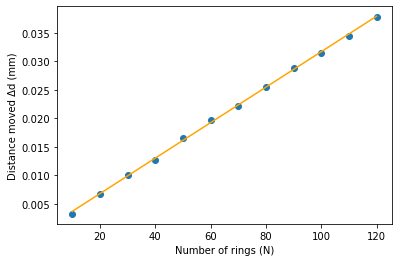
\includegraphics[scale = 0.75]{Figures/laserPlot.png}
    \caption{$\Delta d$ vs $N$ plot for the He-Ne Laser}
    \label{fig:laserplot}
\end{figure}
\begin{figure}[h!]
    \centering
    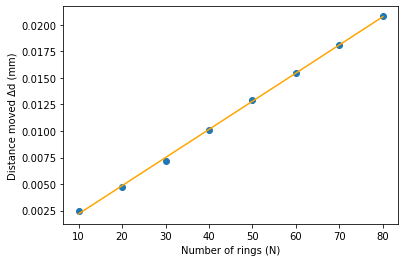
\includegraphics[scale = 0.75]{Figures/lampPlot.png}
    \caption{$\Delta d$ vs $N$ plot for the Na lamp}
    \label{fig:lampplot}
\end{figure}
\section{Calculations}
    \subsection{He-Ne Laser} 
    We first analyse the plot (figure~(\ref{fig:laserplot})) obtained from the table~(\ref{Tab:He-Ne}).
    The five summations for this data-set are as follows:
    \par
    \vspace{0.5cm}
    $S_{x} = \mathlarger{\mathlarger{\sum}} x_{i} = 780$, \hspace{1cm} $S_{y} = \mathlarger{\mathlarger{\sum}} y_{i} = \SI{2.492e-4}{\metre}$,
    \par
    \vspace{0.5cm}
    $S_{xx} = \mathlarger{\mathlarger{\sum}} x_{i}^2 = 65000$, \hspace{1cm} $S_{yy} = \mathlarger{\mathlarger{\sum}} y_{i}^2 = \SI{6.563e-9}{\metre\squared}$,
    \par
    \vspace{0.5cm}
    $S_{xy} = \mathlarger{\mathlarger{\sum}} x_{i}y_{i} = \SI{2.065e-2}{\metre}$
    \par
    \vspace{0.5cm}
    \noindent
    Now the slope is given by 
    \begin{equation}
    \label{eq1}
        m = \dfrac{S S_{xy} - S_{x}S_{y}}{S S_{xx} - S_{x}^2} = \SI{3.113e-7}{\metre} = \SI{311.3}{\nano \metre}
    \end{equation}
    \par
    \vspace{0.5cm}
    \noindent
    $\therefore$ 
    \boxed{$\lambda = 2 \times \SI{311.3}{\nano \metre} = {\SI{622.6}{\nano \metre}}$}
    \subsection{Na Lamp}
    We first analyse the plot (figure~(\ref{fig:lampplot})) obtained from the table~(\ref{Tab:Na}).
    The five summations for this data-set are as follows:
    \par
    \vspace{0.5cm}
    $S_{x} = \mathlarger{\mathlarger{\sum}} x_{i} = 360$, \hspace{1cm} $S_{y} = \mathlarger{\mathlarger{\sum}} y_{i} = \SI{9.180e-5}{\metre}$,
    \par
    \vspace{0.5cm}
    $S_{xx} = \mathlarger{\mathlarger{\sum}} x_{i}^2 = 20400$, \hspace{1cm} $S_{yy} = \mathlarger{\mathlarger{\sum}} y_{i}^2 = \SI{1.349e-9}{\metre\squared}$,
    \par
    \vspace{0.5cm}
    $S_{xy} = \mathlarger{\mathlarger{\sum}} x_{i}y_{i} = \SI{5.245e-3}{\metre}$
    \par
    \vspace{0.5cm}
    \noindent
    Now the slope is given by 
    \begin{equation}
    \label{eq2}
        m = \dfrac{S S_{xy} - S_{x}S_{y}}{S S_{xx} - S_{x}^2} = \SI{2.652e-7}{\metre} = \SI{265.2}{\nano \metre}
    \end{equation}
    \par
    \vspace{0.5cm}
    \noindent
    $\therefore$ 
    \boxed{$\lambda = 2 \times \SI{265.2}{\nano \metre} = \SI{530.4}{\nano \metre}$}
    
\section{Error Analysis}
The error in the slope is given by 
\begin{equation}
\label{eq3}
    \sigma_m = \sigma_y \sqrt{\dfrac{S}{\Delta}}
\end{equation}
\noindent
Here $\sigma_y$ represents the least count of the micrometre and is equalt to $\SI{0.0001}{\milli\metre}$.
    \subsection{He-Ne Lamp}
    We have,
    \begin{equation}
    \label{eq4}
        \Delta = S S_{xx} - S_{x}^2 = 1.716 \times 10^5
    \end{equation}
    Using (\ref{eq1}), (\ref{eq3}) and (\ref{eq4}),  
    \begin{equation}
    \label{eq5}
        \sigma_m = 0.0001 \times \sqrt{\dfrac{12}{1.716 \times 10^5}} = \SI{8.362e-10}{\metre} = \SI{0.8}{\nano \metre}
    \end{equation}
    Now, error in $\lambda$
    \begin{equation}
    \label{eq8}
        \boxed{\sigma_{\lambda} = 2 \times \sigma_{m} = \SI{1.6}{\nano \metre}}
    \end{equation}
    \subsection{Na Lamp}
    We have,
    \begin{equation}
    \label{eq6}
        \Delta = S S_{xx} - S_{x}^2 = 3.360 \times 10^4
    \end{equation}
    Using (\ref{eq2}), (\ref{eq3}) and (\ref{eq6}),  
    \begin{equation}
    \label{eq7}
        \sigma_m = 0.0001 \times \sqrt{\dfrac{8}{3.360 \times 10^4}} = \SI{1.543e-9}{\metre} = \SI{1.5}{\nano \metre}
    \end{equation}
    Now error in $\lambda$
    \begin{equation}
    \label{eq9}
        \boxed{\sigma_{\lambda} = 2 \times \sigma_{m} = \SI{3.0}{\nano \metre}}
    \end{equation}
\section{Results and Discussions}
\begin{enumerate}
    \item From (\ref{eq1}) and (\ref{eq8}), the wavelength of the He-Ne laser is given by $\lambda = 622.6 \pm 1.6$ nm.
    \item From (\ref{eq2}) and (\ref{eq9}), the wavelength of the Na Lamp is given by $\lambda = 530.4 \pm 3.0$ nm.
    \item The obtained value are in reasonable range in case of the He-Ne laser whereas in the case of the Na lamp, the obtained value is considerably off from the literature value.
    \item One of the source of this error/ambiguity could be the way readings have been noted as we can not definitely say when a circular fringe has vanished.
    \clearpage
    \item Fringes of equal inclination were observed using He-Ne laser as shown below
    \begin{figure}[h!]
        \centering
        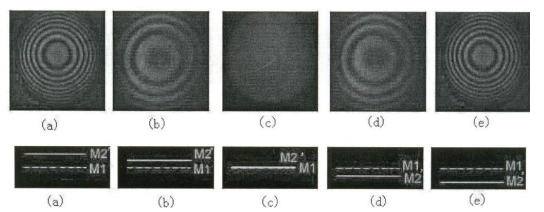
\includegraphics[scale = 0.8]{Figures/fring of equal incl.png}
        \caption{Fringes of equal inclination}
        \label{fig:eqincl}
    \end{figure}
    \item Fringes of equal thickness were observed using He-Ne laser as shown below
    \begin{figure}[h!]
        \centering
        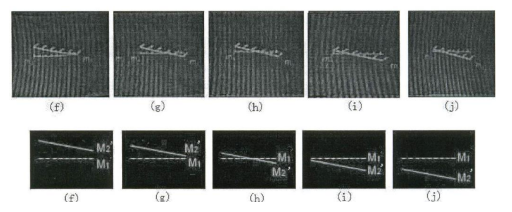
\includegraphics[scale = 0.8]{Figures/fring of equal thick.png}
        \caption{Fringes of equal thickness}
        \label{fig:my_label}
    \end{figure}
\end{enumerate}

\section{Precautions}
\begin{enumerate}
    \item Avoid backlash errors.
    \item Always turn the fine adjustment knob in one direction either clockwise or anti-clockwise.
    \item Direct eye exposure to laser should be avoided.
    \item Observing laser interference fringes by reflecting mirror is prohibited.
    \item Avoid touching any of the optics with bare hand.
\end{enumerate}
\end{document}
